\documentclass{article}
\usepackage[utf8]{inputenc}
\usepackage{minted}
\usepackage{hyperref}
\usepackage{graphicx}
\usepackage[dvipsnames]{xcolor}
\usepackage{comment}

\title{STM32 LoRa and Sigfox Discovery kit B-L072Z-LRWAN1}
\author{cmonaton }
\date{July 2019}

\begin{document}

\maketitle

\section{Introduction}
Le but de ce tuto est d'envoyer la payload de la carte et les coordonnées GPS de la passerelle sur le réseau LoRaWAN.
carte : B-L072Z-LRWAN1

  \begin{figure}[H]
\begin{center}
\advance\leftskip-3cm
\advance\rightskip-3cm
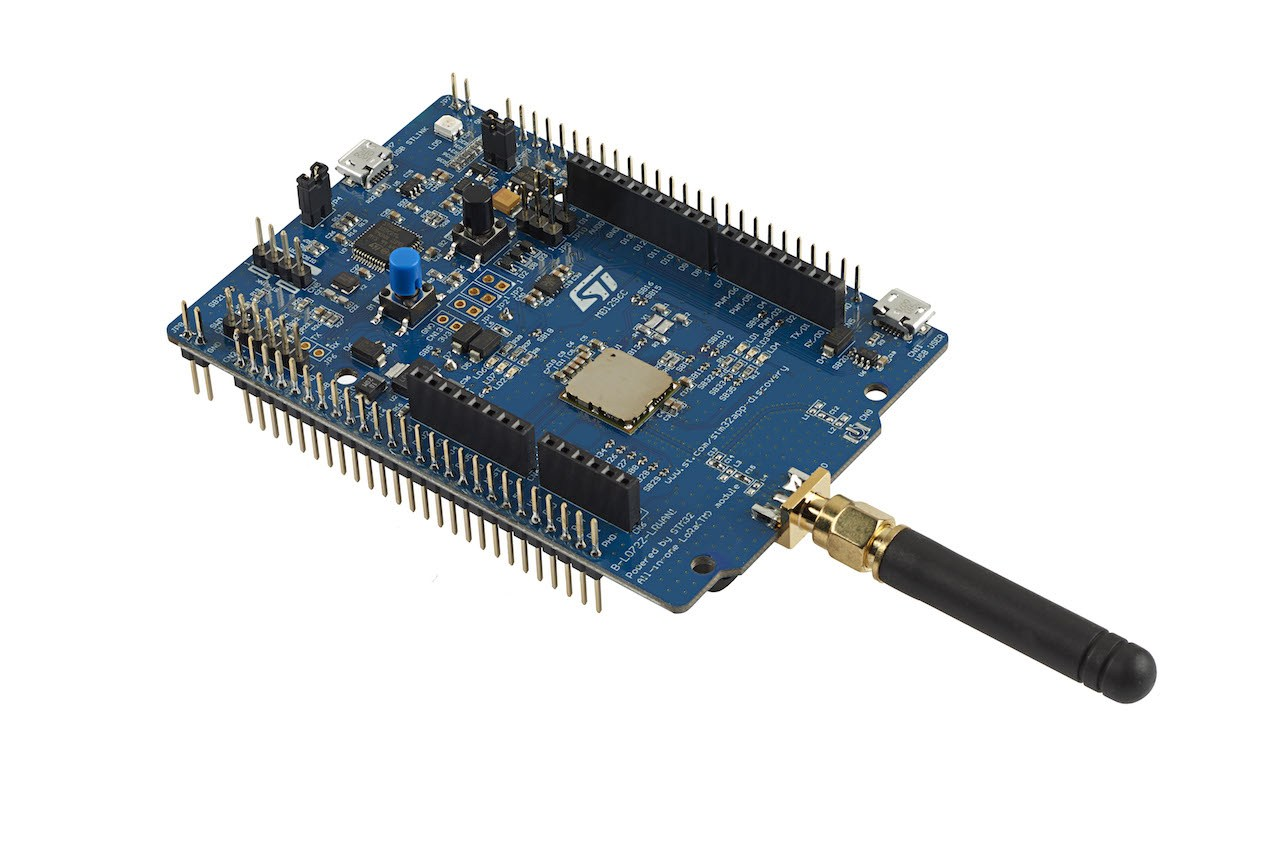
\includegraphics[keepaspectratio=true,scale=0.5]{carte.jpeg}
\label{visina8}
\end{center}\end{figure}

\section{Matériel}
%carte : B-L072Z-LRWAN1


\textcolor{red}{Branchez l'antenne LoRa avant d'alimenter la carte sinon la carte grille}

\section{logiciels à installer}

%\subsection{stm32 workbench}
%\subsubsection{installation}
%Se créer un compte sur OPEN STM32 community.
%Télécharger l'installeur pour linux, l'exécuter



\subsection{STM32 cube IDE }
Télécharger le logiciel sur le site de ST : \url{https://www.st.com/en/development-tools/stm32cubeide.html}\\
Téléchargez le .deb

Se créer au préalable un compte.


\subsection{Installation de STM32 cube programmer}
Ce logiciel permet de télécharger le code sur la carte. \\
\textit{Note}: Il semble impossible d'installer ce programme sous Ubuntu 18.04.3 LTS \\
Sur Ubuntu 16.04.6 LTS
\begin{itemize}
   
\begin{itemize}
   



 \item Avant de lancer l'installer :
\begin{minted}{bash}

sudo apt-get install openjfx

\end{minted}

 \item Se créer un compte et télécharger le logiciel à : \\

\url{https://www.st.com/en/development-tools/stm32cubeprog.html}

\begin{comment}
Lancez l'installer .linux 
\begin{minted}{bash}

./path_of_file.linux

\end{minted}
\end{comment}


\item Téléchargez STSW-LINK007 à : \\ 
\url{https://www.st.com/en/development-tools/stsw-link007.html}


\item Ajouter des règles dans /etc/udev/rules.d

\begin{minted}{bash}

cd /extraction_path/stsw-link007/AllPlatforms/StlinkRulesFilesForLinux

sudo cp *.* /etc/udev/rules.d

sudo udevadm control --reload-rules #ou rebooter le PC


\end{minted}

\end{itemize}

\subsection{Si nécessaire}

\begin{itemize}
    



\item Installer libusb

\begin{minted}{bash}


sudo apt-get install libusb-1.0


\end{minted}

\item  upgrader STlink :

\begin{figure}[H]
\begin{center}
\advance\leftskip-3cm
\advance\rightskip-3cm
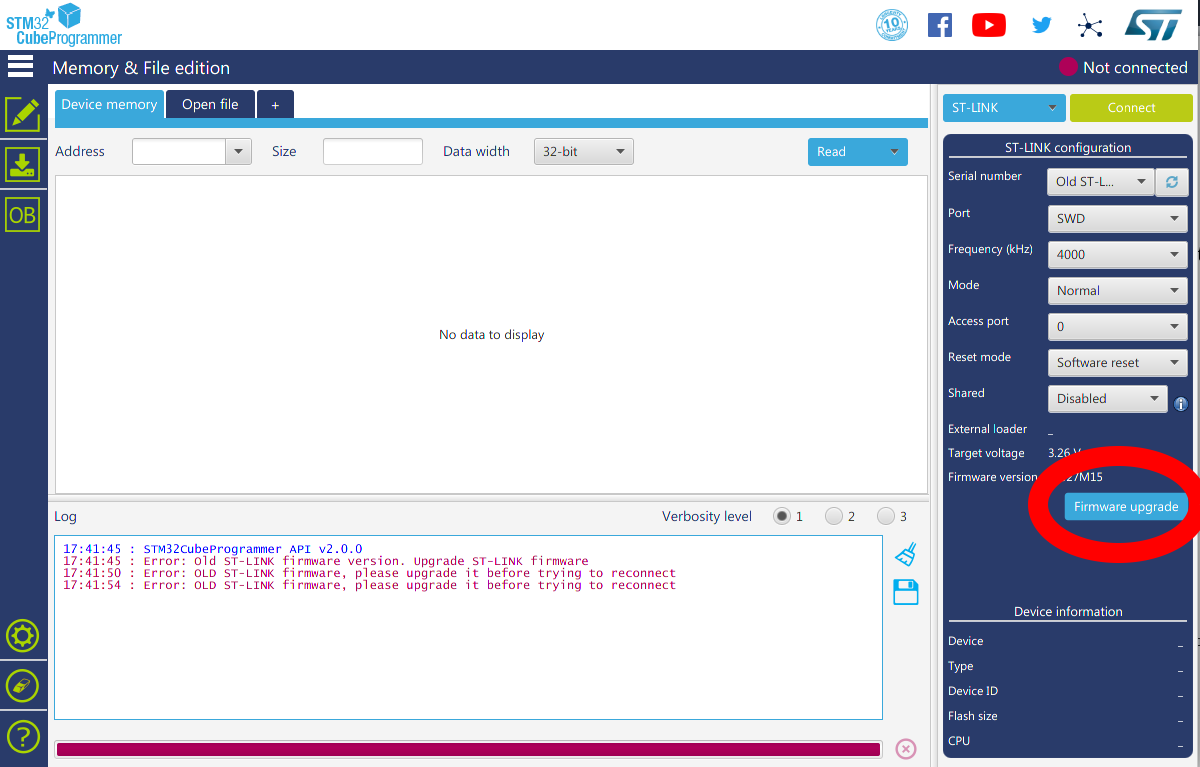
\includegraphics[keepaspectratio=true,scale=0.3]{stlink_upgrade.png}
\label{visina8}
\end{center}\end{figure}



\end{itemize}


\subsection{Application demo}
Le code des applications de démo du kit se trouve à : \\
Demo : \url{https://www.st.com/en/embedded-software/i-cube-lrwan.html}


\subsection{Générer un fichier .bin pour la carte depuis le PC}
Avec STM32 Cube IDE. Voir détail au 4 avec l'exmple du programme End Node.



\subsection{Télécharger le firmware avec STM32 cube programmer}

\begin{enumerate}


      \item Connecter la carte : Parfois la carte ne peut plus se connecter au PC pour flasher le code.
    Explication : le FW bloque le port de STLINK
    Solution : Maintenir appuyé le bouton reset de la carte au moment de la connection avec STM32Cube Programmer

    \item 
    A côté de "device memory" dans un onglet selon l'image, ajouter un fichier et "Download" un fichier .elf ou .bin \\
    
    
    
    
    
    \begin{figure}[H]
\begin{center}
\advance\leftskip-3cm
\advance\rightskip-3cm
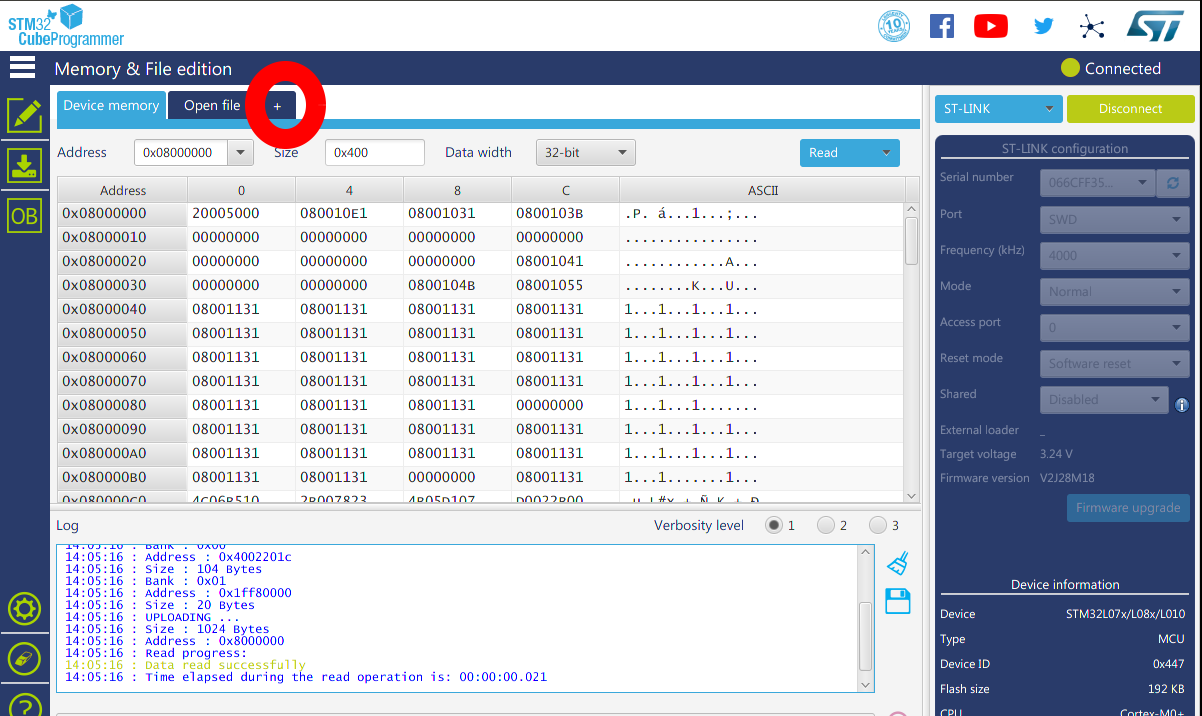
\includegraphics[keepaspectratio=true,scale=0.3]{st_cube_programmer_2.png}
\label{visina8}
\end{center}\end{figure}
    
    
   % \item upgrader le firmware pour STlink quand on flash sur une carte différente.
%    Télécharger la dernière version sur le site de ST, Version : 2.34.25  : \url{https://www.st.com/content/st_com/en/products/development-tools/software-development-tools/stm32-software-development-tools/stm32-programmers/stsw-link007.html} \\
 %   Pour linux, d'après les readme dans  
%    \begin{minted}{bash}
%     /emplacement_extraction/stsw-link007/AllPlatforms/StlinkRulesFilesForLinux
    
%    \end{minted}
     
%    \begin{minted}{bash}
%    java -jar STLinkUpgrade.jar #dans le bon dossier
%    #et :
%    sudo cp *.* /etc/udev/rules.d
%    \end{minted}
   
\end{enumerate}



\section{Utiliser un terminal série pour communiquer avec la carte}


Sur Ubuntu :
localiser le port USB sur lequel la carte est branchée : 
\begin{enumerate}



\item Avec dmesg :


\begin{minted}{bash}
dmesg | grep tty 
\end{minted}{bash}
dans mon cas : ttyACM0: USB ACM device



%\item avec tkdiff
%\begin{minted}{bash}
%sudo apt-get install tkdiff

%cd ~
%touch log.txt log2.txt
%ls /dev > log.txt
%#débrancher la carte
%ls /dev > log2.txt
%tkdiff log.txt log2.txt
%\end{minted}
\end{enumerate}

\subsection{Liaison série avec la carte :}

\begin{enumerate}



\item PuTTy : ubuntu : 
\begin{minted}{bash}
sudo apt-get install putty
\end{minted}
Choisir le mode série, choisir le port de la carte, /dev/ttyACM0 dans mon cas, baudrate 115200

\item
Avec Minicom : sudo apt-get install minicom \\
Configurer la liason : sudo minicom -s

Désactiver les contrôles de flux logiciels et matériels
Baudrate : 115200

%Penser à sauvegarde la configuration pour ne pas avoir à la re-entrer à chaque fois

Pour quitter minicom : ctrl + A puis q

\end{enumerate}

%Envoyer des commandes AT à la carte :



\section{Lire les messages envoyés sur LoRa server}

Obtenir des identifiants LoRa server, contacter : didier.donsez@univ-grenoble-alpes.fr

\url{https://lora.campusiot.imag.fr/#/login}

\subsection{Avec l'exemple End Node  du software demo -cube-lrwan (URL plus haut)}

\subsubsection{Etape 1 : Flasher le programme sur la carte}

\begin{enumerate}
    


\item Ouvrir le projet avec STM32Cube IDE \\ chemin :
\begin{minted}{bash}
/home/username/STM32CubeExpansion_LRWAN
_V1.2.1/Projects/B-L072Z-LRWAN1/Applications/LoRa/End_Node
\end{minted}

en utilisant : File, Open project from filesystem \\
Puis bouton build all \\
\item


Le fichier binaire se trouve à :

\begin{minted}{bash}
chemin_projet/Debug/NomDuProjet.bin
\end{minted}


\begin{comment}
Trouver l'emplacement du fichier .bin généré : 
\begin{minted}{bash}
find /home | grep -w .bin
\end{minted}
.elf, le fichier .bin est dans le même dossier que le .elf
\end{comment}




\item Ouvrir STM32Cube Programmer :
Connecter la carte cf \textit{Flasher le FW avec STM32 cube programmer} \\
Flasher le .bin. \\
Déconnecter la carte avec le bouton disconnect \\
Parfois il faut supprimer les anciens fichiers .bin et .elf dans

\begin{minted}{bash}
/extraction_path/STM32CubeExpansion_LRWAN_V1.2.2/Projects/B-L072Z-LRWAN1/
Applications/LoRa/project_name/SW4STM32/mlm32l07x01/Debug

\end{minted}

pour avoir les .bin et .elf de la dernière compilation. \\
Ouvrir PuTTy et connecter la carte cf  \textit{Utiliser  un  terminal  série  pour  commandes AT et communiquer avec la carte} \\


\subsubsection{Pour ouvrir les ports ttyACM0 et ttyACM1 }

\textbf{Solution temporaire} 


\begin{minted}{bash}
sudo chmod 666 /dev/ttyACM0
\end{minted}
Il faut le entrez cette commande souvent. \\
\textbf{Solution permanente}\\

Créer un fichier dans son home

\begin{minted}{bash}
50-myusb.rules
\end{minted} 

l'éditer : 

\begin{minted}{bash}
KERNEL=="ttyACM[0-9]*",MODE="0666"
\end{minted}

Puis copiez ce fichier dans /etc/udev/rules.d/ et redémarrez votre PC. \\

\begin{minted}{bash}
 sudo cp 50-myusb.rules /etc/udev/rules.d
\end{minted}
C'est suffisant pour ne plus avoir à réouvrir les ports manuellement. Cependant, n'importe quel dispositif usb connecté au PC a maintenant le droit d'écriture sur le PC. \\

Pour plus de sécurité ajouter ces lignes dans ce fichier :

\begin{minted}{bash}
ACTION=="add", KERNEL=="ttyACM[0-9]*", ATTRS{idVendor}=="xxxx", 
ATTRS{idProduct}=="yyyy", MODE="0666"
\end{minted}
 
 Pour déterminer idVendor et idProduct des cartes tapez lsusb avant et après avoir connecter la carte. \\

 Dans mon cas avant et après avoir branché une carte lopy4 :
 
 \begin{figure}[H]
\begin{center}
\advance\leftskip-3cm
\advance\rightskip-3cm
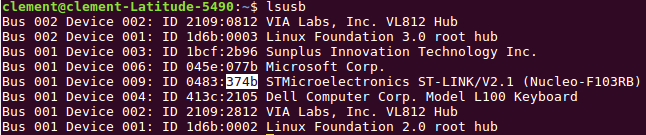
\includegraphics[keepaspectratio=true,scale=0.5]{lsusb.png}
\label{visina8}
\end{center}\end{figure}

idProduct = 0483  \\
idVendor= 374b \\

Pour ajouter d'autres appareils, copier coller ces lignes en changeant idProduct et idVendor. \\


%ans un terminal \begin{minted}{bash}
%sudo chmod 666 /dev/ttyACM0
%\end{minted} \\



\end{enumerate}



\subsubsection{Etape 2 : Enregitrer la carte sur LoRa server et établir la connexion entre le serveur et la carte}

Voir également ce tuto : 
\url{https://github.com/CampusIoT/tutorial/blob/master/loraserver/README-app.md} \\

Sur le site loraserver \url{https://lora.campusiot.imag.fr/#/login}\\
\begin{enumerate}
    


\item Créer une application bouton Applications à gauche
Champs Nom, description : pas d'importance.
Service profile : choisir DEFAULT


 \begin{figure}[H]
\begin{center}
\advance\leftskip-3cm
\advance\rightskip-3cm
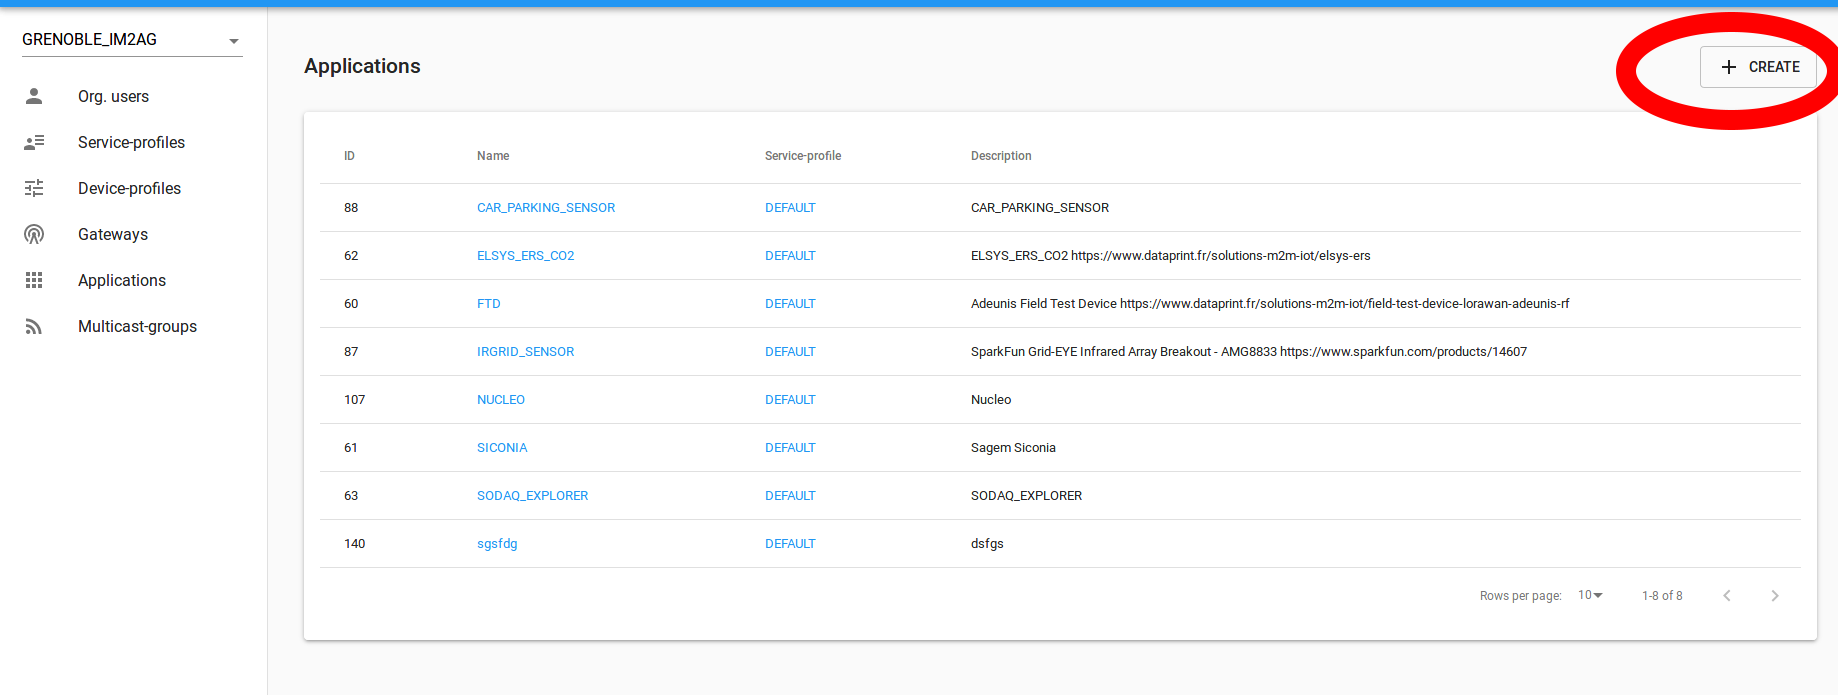
\includegraphics[keepaspectratio=true,scale=0.3]{loraserver_app_create.png}
\label{visina8}
\end{center}\end{figure}

\begin{figure}[H]
\begin{center}
\advance\leftskip-3cm
\advance\rightskip-3cm
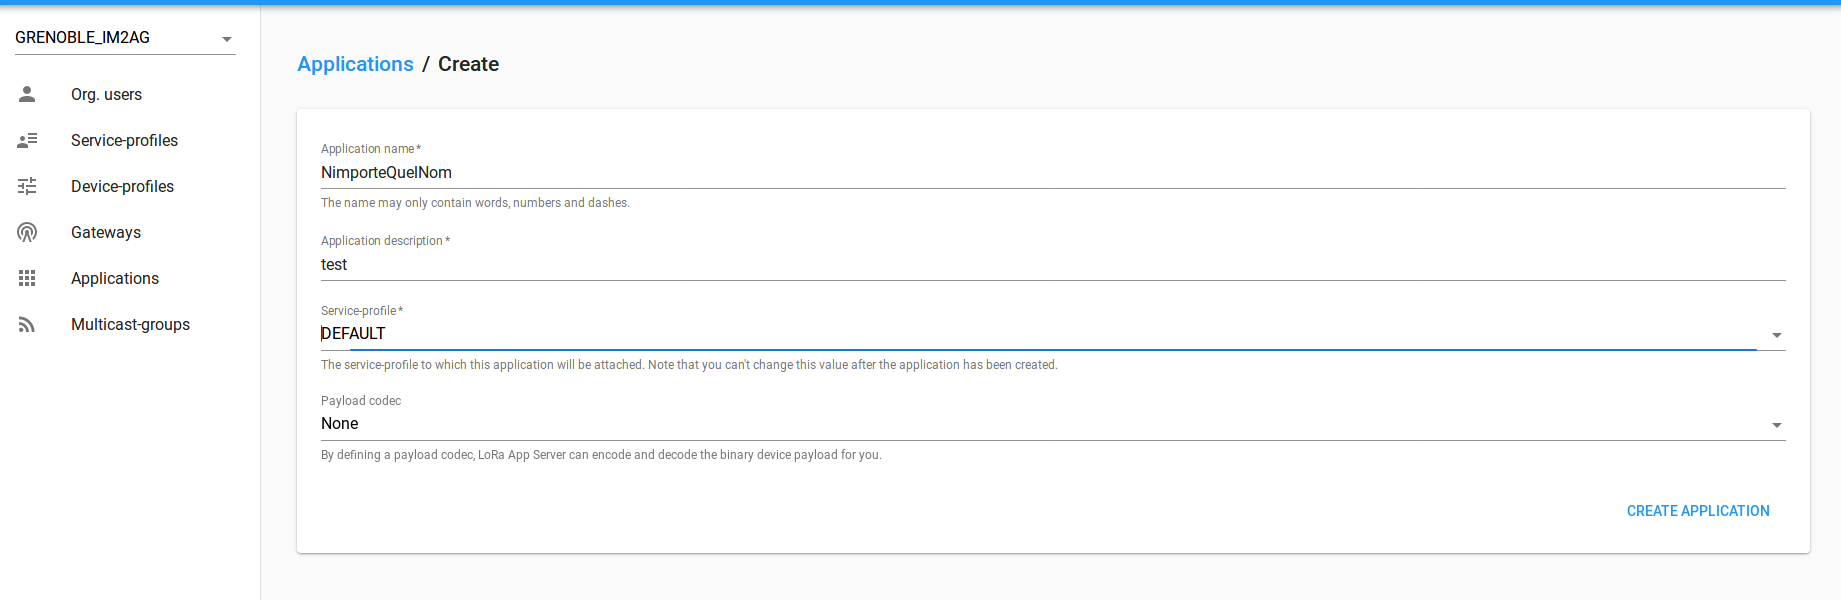
\includegraphics[keepaspectratio=true,scale=0.3]{loraserver_application_form.png}
\label{visina8}
\end{center}\end{figure}




\subsubsection{Code}
Dans le fichier 
\begin{minted}{bash}
/extraction_path/STM32CubeExpansion_LRWAN_V1.2.2/Projects/STM32L073RZ-Nucleo/
Applications/LoRa/End_Node/LoRaWAN/App/inc/Commissioning.h
\end{minted}
Définir STATIC\_DEVICE\_EUI  à 1 \\


Entrer le DEVUI de la carte.\\
Le devEUI est par défaut 0101010101010101 \\
\item Créer un device dans l'application

\begin{figure}[H]
\begin{center}
\advance\leftskip-3cm
\advance\rightskip-3cm
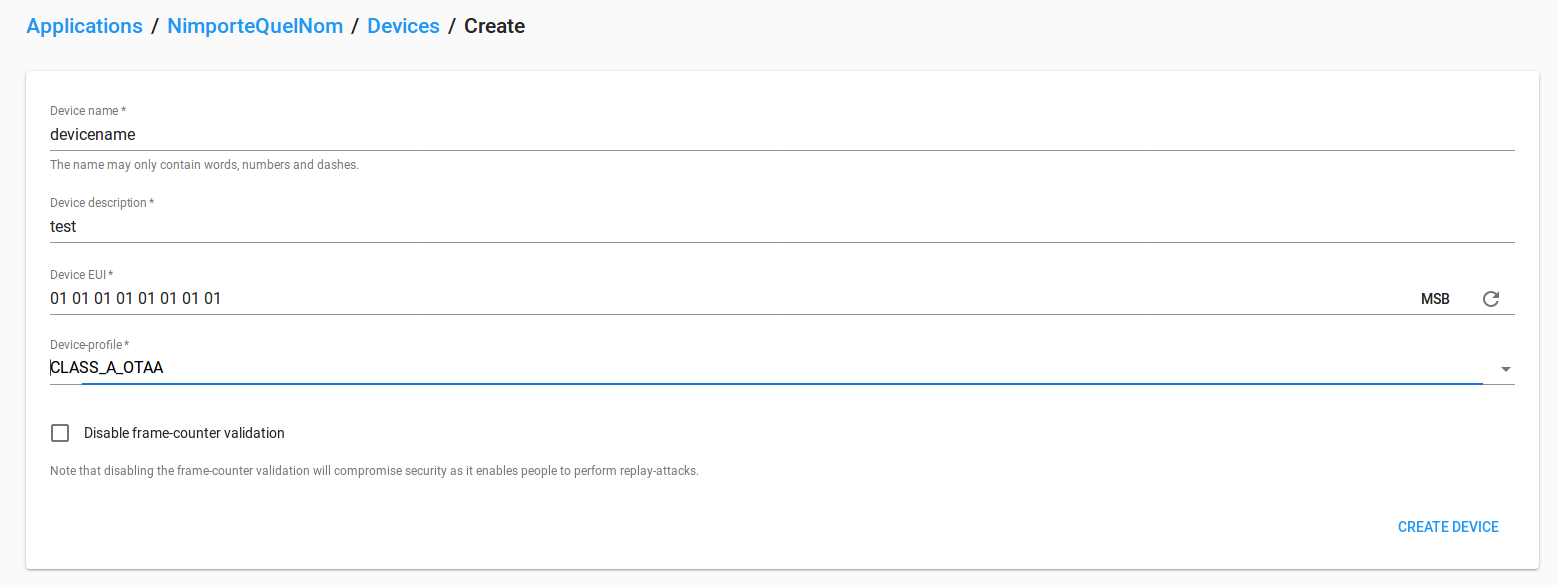
\includegraphics[keepaspectratio=true,scale=0.3]{loraserver_create_device.png}
\label{visina8}
\end{center}\end{figure}


Compilez et téléchargez le code sur la carte.\\


Appuyer sur le bouton reset de la carte \\

Le DevEUI de la carte et l'App Key devraient s'afficher selon l'image.

 \begin{figure}[H]
\begin{center}
\advance\leftskip-3cm
\advance\rightskip-3cm
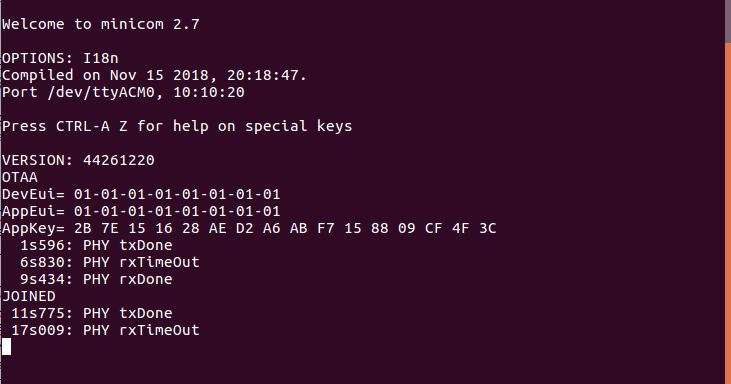
\includegraphics[keepaspectratio=true,scale=0.4]{version_deveui_bl072Z.png}
\label{visina8}
\end{center}\end{figure}

Device profile : CLASS\_A\_OTAA

\item Entrer l'app key dans la clé KEY(OTAA)

\item Appuyer sur Reset de la carte

\item La carte va se connecter et les trames sont visibles depuis l'onglet Live Device Data

\begin{figure}[H]
\begin{center}
\advance\leftskip-3cm
\advance\rightskip-3cm
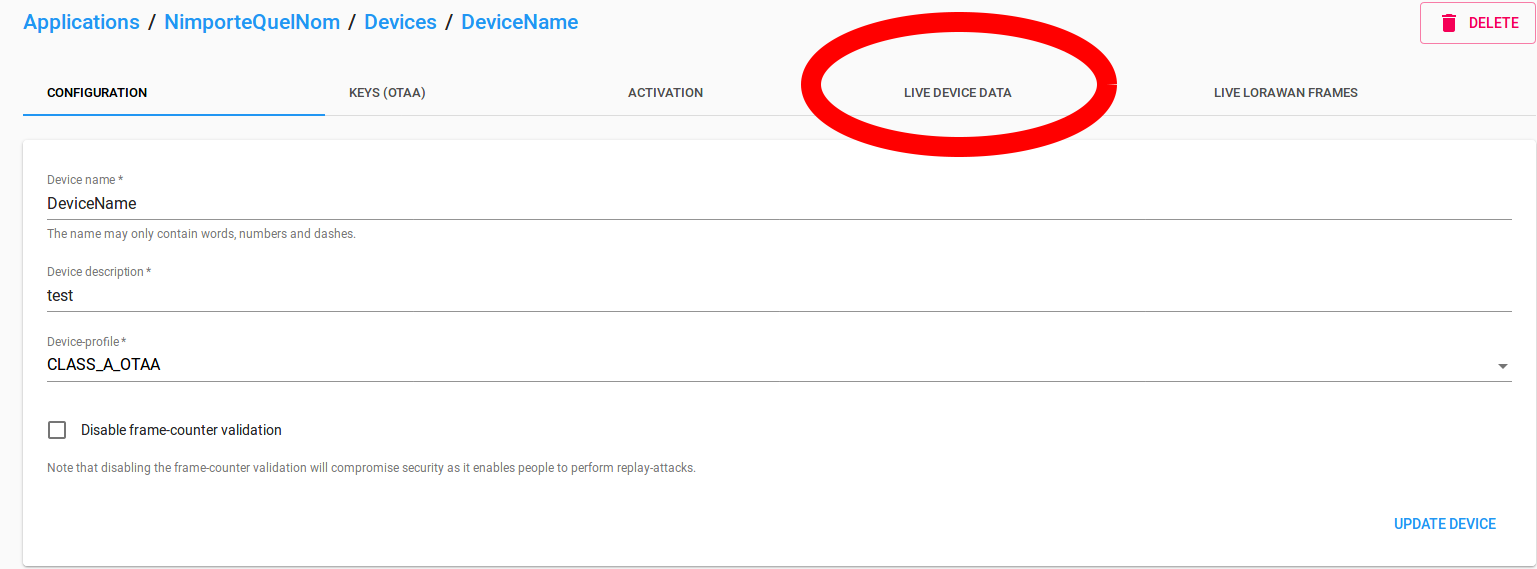
\includegraphics[keepaspectratio=true,scale=0.3]{loraserver_device_data.png}
\label{visina8}
\end{center}\end{figure}




info envoyées : Coordonnées GPS de la passerelle, payload de la carte
\end{enumerate}

\begin{figure}[H]
\begin{center}
\advance\leftskip-3cm
\advance\rightskip-3cm
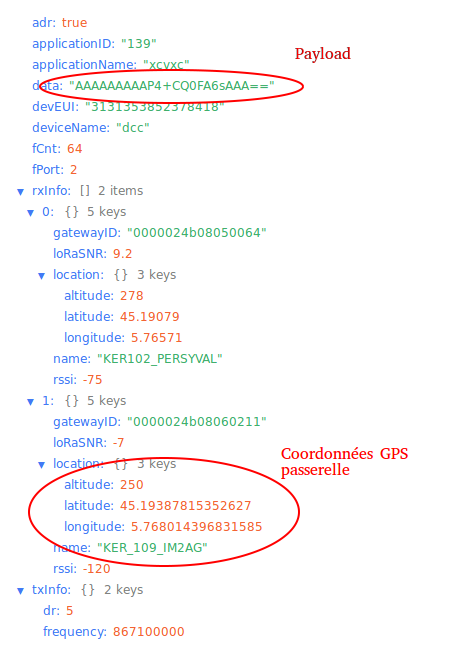
\includegraphics[keepaspectratio=true,scale=0.4]{data.png}
\label{visina8}
\end{center}\end{figure}




%Dans le fichier Commissioning.h :

%Renseigner le champ LORAWAN\_NETWORK\_ID, i'ID s'obtient sur le site loraserver

%Bien penser à rebuilder l'appli puis re-télécharger le FW sur la carte.

%Activer la carte


%\subsection{Obtenir une appkey et un Deveui : cas du STM32 LoRa and Sigfox discovery kit}
%D'après le feuillet :





%\section{Mettre en plce une gateway pycom LoPy 4}

%Suivre le tuto : https://github.com/CampusIoT/tutorial/blob/master/loraserver/README-gateway.md






\end{document}
